\subsection{PCA}
EL primer modelo utilizado para intentar clasificar los datos será el de Analisis de Componentes Principales. Para ello utilizamremos dos algoritmos basados en aprendisaje Hebbiano y reduciremos las instancias de entrenamiento a 3 dimenciones. Lo que esperamos observar es que aquellas instancias que pertenecen a una misma clase de empresa se encuentran cercas unas de otras, pudiendo observar \"nuves\" de puntos bien definidas.

\subsubsection{Implementación}

En particular los algoritmos utilizados serán los de $Oja$ y $Sanger$. Teniendo una complegidad computacional identica y siendo los algoritmos muy similares, lo distintivo entre estos dos metodos es que $Sanger$ ordenará las componentes prinsipales de mayor a menor de acuerdo a sus autovalores mientras que $Oja$ no.

El pseodocodigo utilizado para aprendisaje del algoritmo $Oja$ será:

\begin{algorithm}
\begin{algorithmic}[1]\parskip=1mm
 \caption{ Algoritmo De Oja}
 \STATE{Para toda instancia de entrenamiento, x}
 \STATE{\quad $y = x.W$}
 \STATE{\quad $\tilde x = y.W^T$}
 \STATE{\quad $\Delta W = learning\_rate ((x - \tilde x)^T . y$}
\end{algorithmic}
\end{algorithm}

Mientras que el de $Sanger$

\begin{algorithm}
\begin{algorithmic}[1]\parskip=1mm
 \caption{ Algoritmo De Sanger}
 \STATE{U = Matriz Triangular Superior Con 1s}
 \STATE{Para toda instancia de entrenamiento, x}
 \STATE{\quad $y = x.W$}
 \STATE{\quad $\tilde x = W(y^T.U)$}
 \STATE{\quad $\Delta W = learning\_rate ((x^T - \tilde x) . y$}
\end{algorithmic}
\end{algorithm}

Utilizando el paquete numpy de python es posible traducir este codigo de manera casi exacta y de esa manera aprovechar las optimizaciones matriciales que se realizan sobre los datos.

\subsubsection{Experimentación}

Para la experimentación entrenamos la red con parte del set de datos que nos fue entregado, una vez realizado esto graficaremos los mismo en el espacio marcando con colores cual era la categoría real de cada punto. De esta manera esperamos distinguir nubes de puntos de un mismo color cercanos entre ellos y alejados de aquellos que pertenecen a otras categorías. Como primera instancia quisimos ver que el algormitmo convería realmente a una solución y la manera en que lo realizaba. En el siguiente apartado presentaremos como convergió la solución en cada caso para valores que a priori daban resultados aceptables.

\subsubsection{Sanger}

Con learning rate igual a $0.1$ y $100$ epocas, y una matriz inicial de pesos normal con media 0 y varianza $1/\sqrt(cantidad_neuronas_entrada)$ obtuvimos los siguientes resultados:

\begin{figure}[h!]
\centering
  \centering
  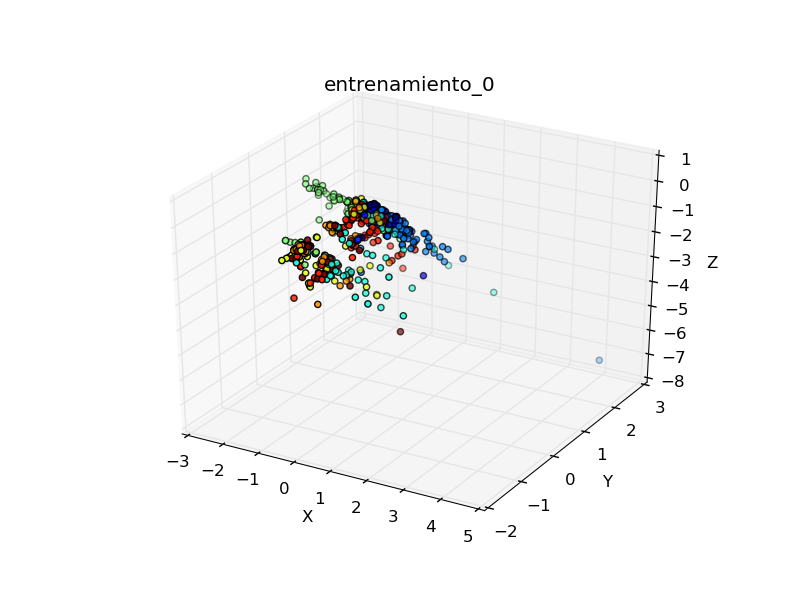
\includegraphics[width=.6\linewidth]{img/convergencia_oja/entrenamiento_0.png}
\caption{Sin entrenar}
\label{fig:test}
\end{figure}

En primer instancia, con la matriz sin haber sido entrenada los datos no presentan ningun ordenamiento adecuado.

\pagebreak

Luego de $25$ epocas se observa: 

\begin{figure}[h!]
  \centering
  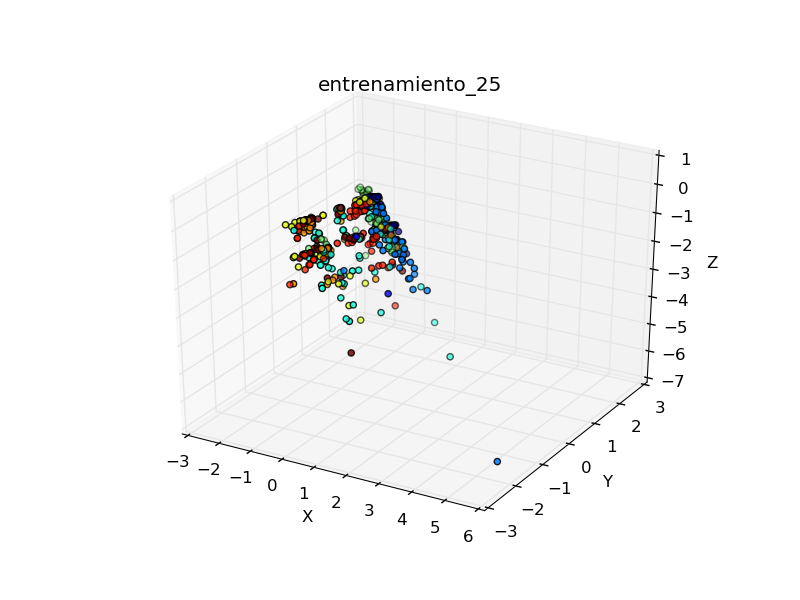
\includegraphics[width=.6\linewidth]{img/convergencia_oja/entrenamiento_25.png}
\caption{25 epocas}
\label{fig:test}
\end{figure}

Ya aquí se presenta cierto ordenamiento...

\pagebreak

Para 50 y 75 epocas puede observarse:

\begin{figure}[h!]
\centering
\begin{subfigure}{.5\textwidth}
  \centering
  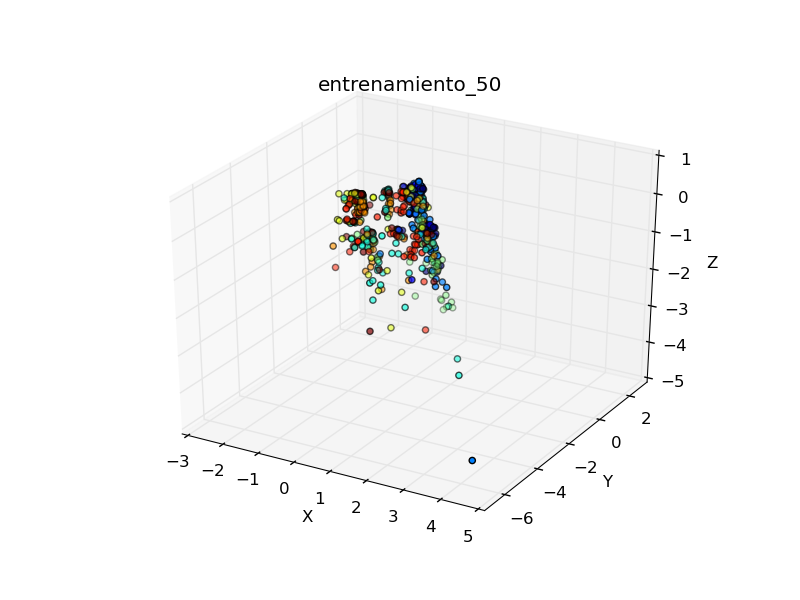
\includegraphics[width=.9\linewidth]{img/convergencia_oja/entrenamiento_50.png}
  \caption{50 epocas}
  \label{fig:sub1}
\end{subfigure}%
\begin{subfigure}{.5\textwidth}
  \centering
  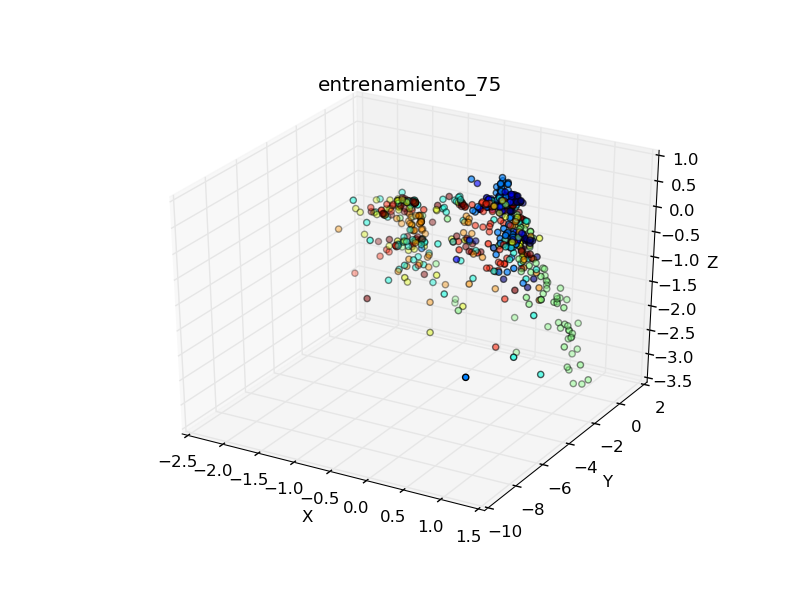
\includegraphics[width=.9\linewidth]{img/convergencia_oja/entrenamiento_75.png}
  \caption{75 epocas}
  \label{fig:sub2}
\end{subfigure}
\caption{50 y 75 epocas}
\label{fig:test}
\end{figure}

Finalmente para 100 epocas puede verse que los datos ya presentan un grado mayor de ordenamiento:

\begin{figure}[h!]
	\centering
	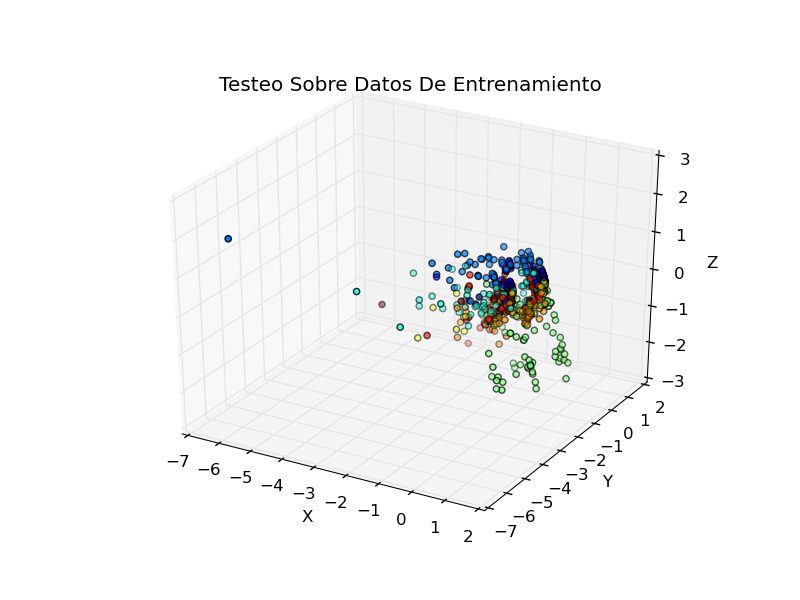
\includegraphics[width=.6\linewidth]{img/convergencia_oja/entrenamiento_100.png}
	\captionof{figure}{A figure}
	\label{fig:test1}
	\centering
\end{figure}

Ya aquí puede observarse un mayor grado de clusterización. Los puntos verdes y azules estan marcadamente a los costados del graficos.

\pagebreak

\subsection{Sanger}

Realizando algo parecido para el algormitmo de sanger, podemos observar los siguentes resultados:

\begin{figure}[h!]
  \centering
  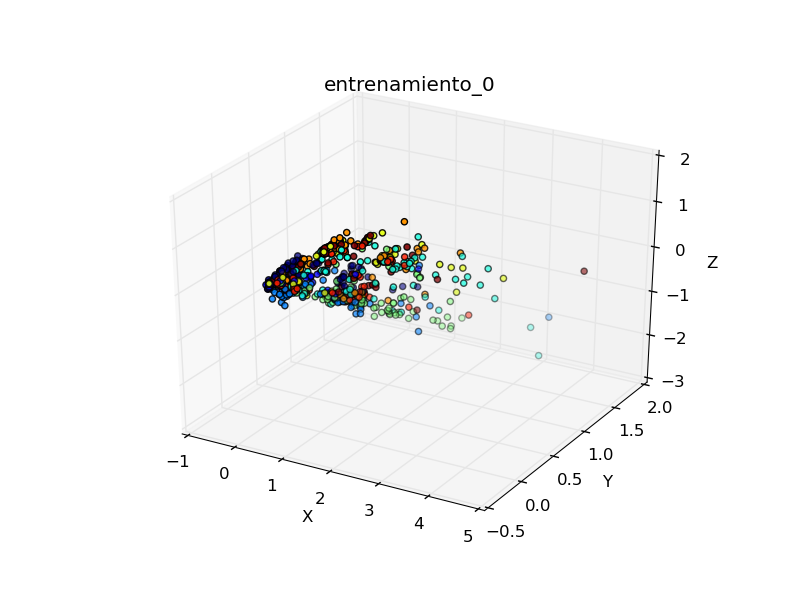
\includegraphics[width=.6\linewidth]{img/convergencia_sanger/entrenamiento_0.png}
\caption{0 epocas}
\label{fig:test}
\end{figure}

Ningun ordenaimento.

\begin{figure}[h!]
  \centering
  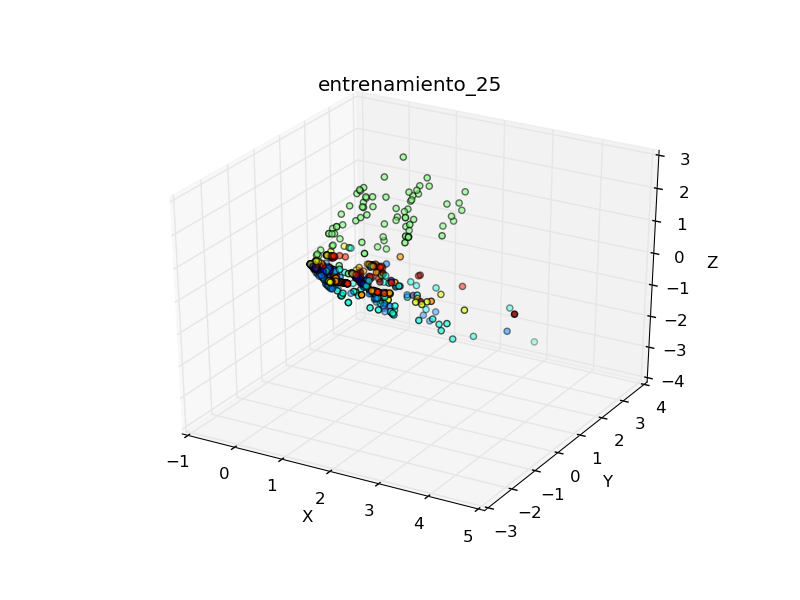
\includegraphics[width=.6\linewidth]{img/convergencia_sanger/entrenamiento_25.png}
\caption{25 epocas}
\label{fig:test}
\end{figure}


\begin{figure}[h!]
\centering
\begin{subfigure}{.5\textwidth}
  \centering
  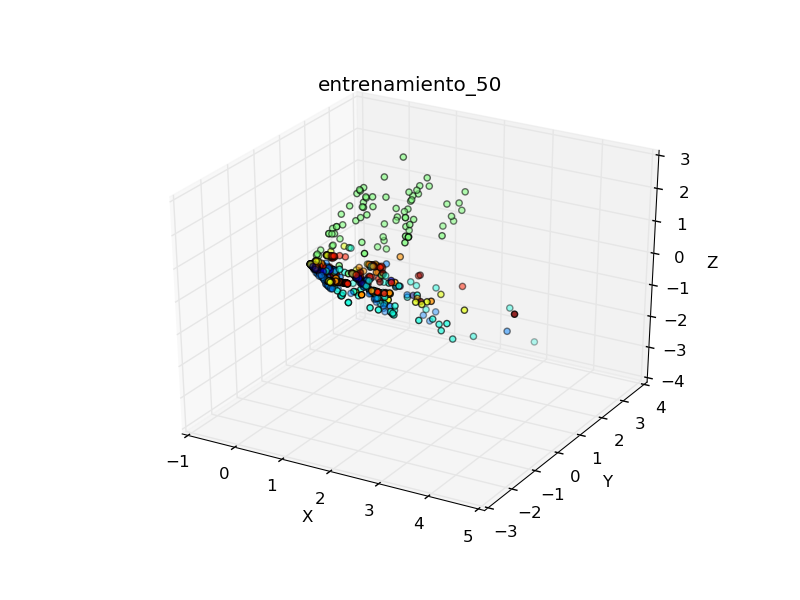
\includegraphics[width=.4\linewidth]{img/convergencia_sanger/entrenamiento_50.png}
  \caption{A subfigure}
  \label{fig:sub1}
\end{subfigure}%
\begin{subfigure}{.5\textwidth}
  \centering
  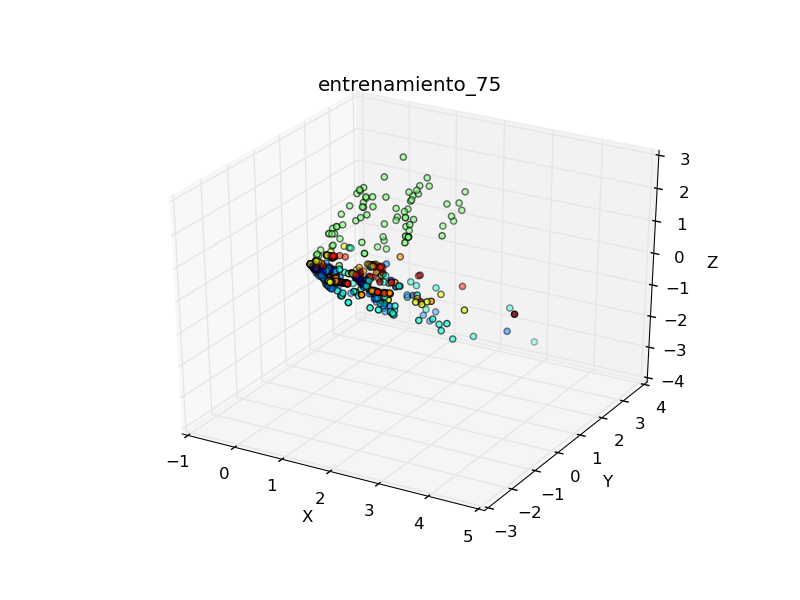
\includegraphics[width=.4\linewidth]{img/convergencia_sanger/entrenamiento_75.png}
  \caption{A subfigure}
  \label{fig:sub2}
\end{subfigure}
\caption{A figure with two subfigures}
\label{fig:test}
\end{figure}

\begin{figure}[h!]
	\centering
	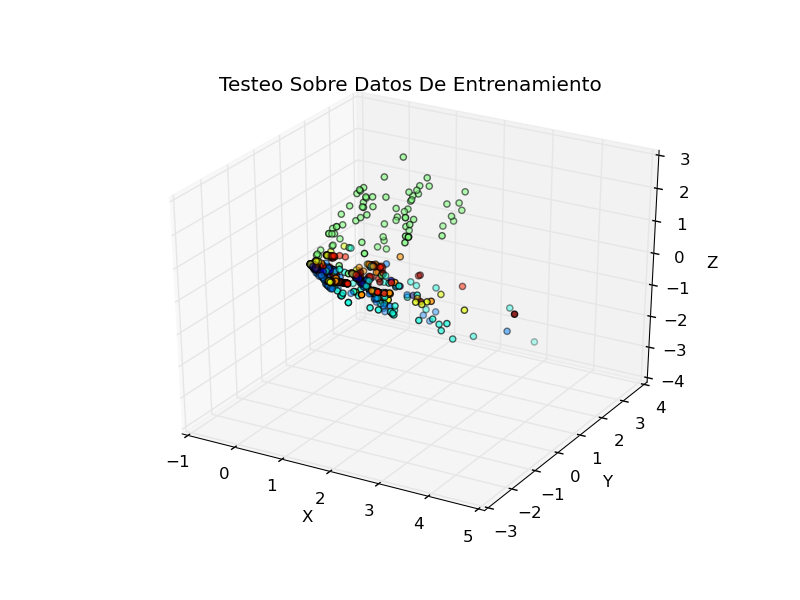
\includegraphics[width=.6\linewidth]{img/convergencia_sanger/entrenamiento_100.png}
	\captionof{figure}{A figure}
	\label{fig:test1}
	\centering
\end{figure}

%Neural Networks Haykin
% In Chatterjee et al. (1998), the convergence properties of the GHA algorithm
% described in Eq. (8.91) are investigated. The analysis presented therein shows that
% increasing  leads to faster convergence and larger asymptotic mean-square error, which
% is intuitively satisfying. In that paper, the tradeoff between the accuracy of computation
% and speed of learning is made explicit.



\subsection{Mapeo de Características}

En este apartado construiremos un modelo de mapeo de caracteristicas auto-organizado con la intención de clasificar los documentos en un arreglo de dos dimenciones. Para ello utilizaremos el algoritmo de Kohonen sobre los datos de entrenamiento y una vez que la red haya convergido, intentaremos darle sentido a los resultados.

\subsubsection{Implementación}

El algoritmo basico utilizado será el visto en clases, que basicamente se divide en:

\begin{algorithm}
\begin{algorithmic}[1]\parskip=1mm
 \caption{ Activación(x)}
 \STATE{$\tilde y = \norm{x^T -MatrizDePesos}$}
 \STATE{$y = (\tilde y == min(\tilde y))*1.0$}
 \STATE{retornar $y$}
\end{algorithmic}
\end{algorithm}

% y_raya = np.linalg.norm(x - self.weights.T,axis=1)
% y = (y_raya == np.amin(y_raya))*1.0
% return y

\begin{algorithm}
\begin{algorithmic}[1]\parskip=1mm
 \caption{ correccion(x,y)}
 \STATE{$j^* = np.nonzero(y)$}
 \STATE{$D = \Delta(j^*,epoca)$}
 \STATE{$\Delta pesos = learning_rate(epoca).D(x^T-self.weights)$}
 \STATE{$MatrizDePesos = MatrizDePesos + \Delta pesos$}
\end{algorithmic}
\end{algorithm}

% j_ast = np.nonzero(y)
% j_ast = j_ast[0][0]
% D = self.delta_func(j_ast,epoca)
% #Cambiado el learning rate adaptativo se deberian obtener diferentes resultados
% delta_weights = learning_rate.calcular(epoca) * D * (x - self.weights.T).T
% self.weights += delta_weights
% return

\subsubsection{Convergencia Kohonen}

\begin{figure}[h!]
\centering
\begin{minipage}{.15\textwidth}
  \centering
  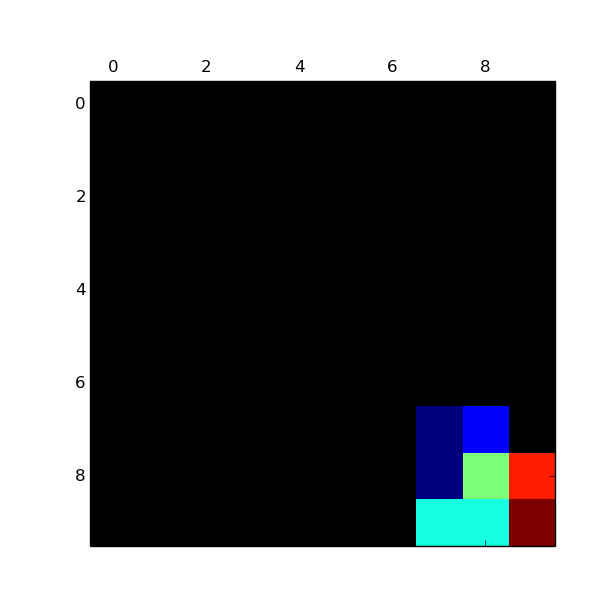
\includegraphics[width=.9\linewidth]{img/convergencia_kohonen/entrenamiento_0.png}
  \captionof{figure}{0\%}
  \label{fig:test1}
\end{minipage}%
\begin{minipage}{.15\textwidth}
  \centering
  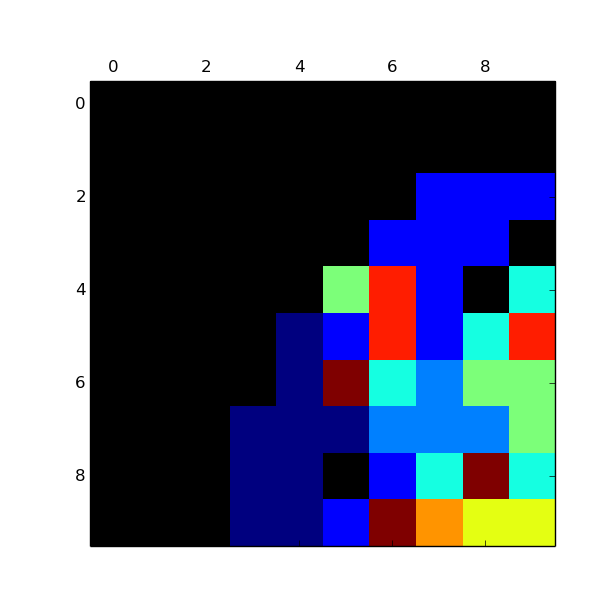
\includegraphics[width=.9\linewidth]{img/convergencia_kohonen/entrenamiento_25.png}
  \captionof{figure}{25\%}
  \label{fig:test2}
\end{minipage}
\begin{minipage}{.15\textwidth}
  \centering
  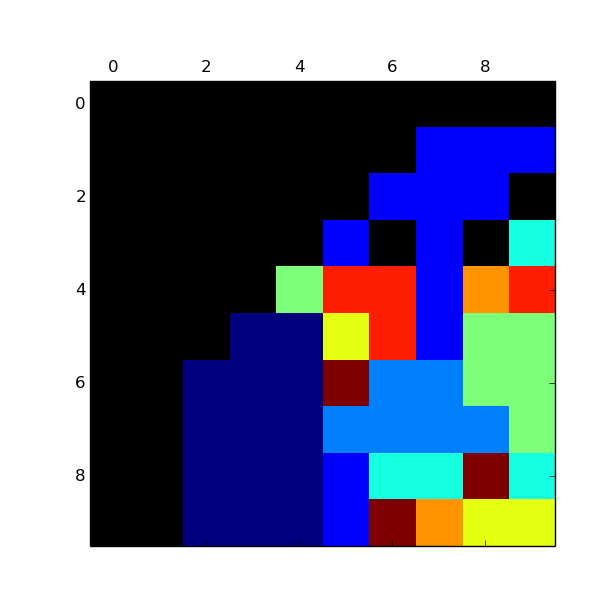
\includegraphics[width=.9\linewidth]{img/convergencia_kohonen/entrenamiento_50.png}
  \captionof{figure}{50\%}
  \label{fig:test2}
\end{minipage}
\begin{minipage}{.15\textwidth}
  \centering
  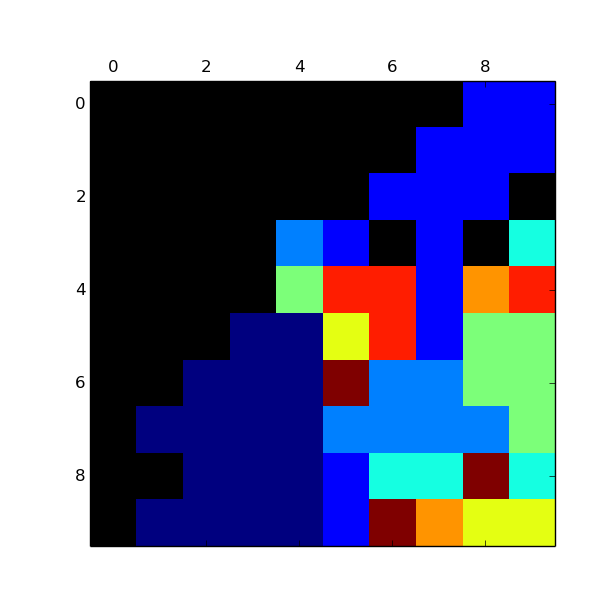
\includegraphics[width=.9\linewidth]{img/convergencia_kohonen/entrenamiento_75.png}
  \captionof{figure}{75\%}
  \label{fig:test2}
\end{minipage}
\begin{minipage}{.15\textwidth}
  \centering
  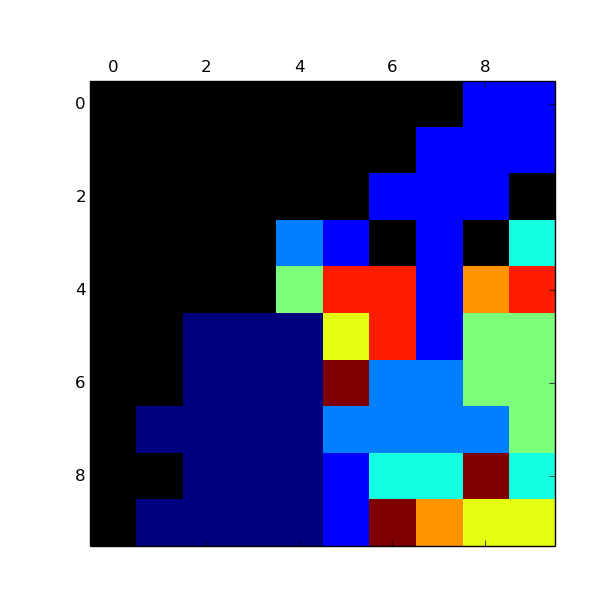
\includegraphics[width=.9\linewidth]{img/convergencia_kohonen/entrenamiento_100.png}
  \captionof{figure}{100\%}
  \label{fig:test2}
\end{minipage}
\end{figure}